% \iffalse
\let\negmedspace\undefined
\let\negthickspace\undefined
\documentclass[journal,12pt,onecolumn]{IEEEtran}
\usepackage{cite}
\usepackage{amsmath,amssymb,amsfonts,amsthm}
\usepackage{algorithmic}
\usepackage{graphicx}
\usepackage{textcomp}
\usepackage{xcolor}
\usepackage{txfonts}
\usepackage{listings}
\usepackage{enumitem}
\usepackage{mathtools}
\usepackage{gensymb}
\usepackage{comment}
\usepackage[breaklinks=true]{hyperref}
\usepackage{tkz-euclide} 
\usepackage{listings}
\usepackage{gvv}    
\usepackage{enumitem}
\usepackage{amsmath}
\usepackage{enumerate}% http://ctan.org/pkg/enumerate
\def\inputGnumericTable{}                                 
\usepackage[latin1]{inputenc}                                
\usepackage{color}                                            
\usepackage{array}                                            
\usepackage{longtable}                                       
\usepackage{calc}                                             
\usepackage{multirow}                                         
\usepackage{hhline}                                           
\usepackage{ifthen}                                           
\usepackage{lscape}
\usepackage{tabularx}

\newtheorem{theorem}{Theorem}[section]
\newtheorem{problem}{Problem}
\newtheorem{proposition}{Proposition}[section]
\newtheorem{lemma}{Lemma}[section]
\newtheorem{corollary}[theorem]{Corollary}
\newtheorem{example}{Example}[section]
\newtheorem{definition}[problem]{Definition}
\newcommand{\BEQA}{\begin{eqnarray}}
\newcommand{\EEQA}{\end{eqnarray}}
\newcommand{\define}{\stackrel{\triangle}{=}}
\theoremstyle{remark}
\newtheorem{rem}{Remark}
\begin{document}
\bibliographystyle{IEEEtran}
\vspace{3cm}

\title{NCERT-discrete : 10.5.3 - 2}
\author{EE23BTECH11025 - Anantha Krishnan $^{}$% <-this % stops a space
}
\maketitle
\bigskip



\section{question}
\vspace{0.5cm}
Find the sums given below:
\begin{enumerate}
    \item  7 + 10.5 + 14 ... + 84
    \item  34 + 32 + 30 ... + 10
    \item  -5 + -8 + -11 ... -230
\end{enumerate}

 \vspace{0.5cm}

\begin{center}
\begin{tabular}{ |c|c|c| } 
 \hline
 Symbols & Description & Values    \\
 \hline
  \small $d_i$ & \small Common Difference & 3.5, -2, -3\\
  \small $x_i(n)$ & \small Sequence  &  \scriptsize ($x_i(0)$ +$nd_i$)$u_{(k)}$\\
     \small $X_i(z)$ & \small Z-Transform of $x_i(n)$ & \scriptsize 2$x_i(0)(1-z)^{-1}+(d_i)z(1-z)^{-2}$ \\
     \small $S_i(k)$ & \scriptsize Sum of k-terms in $i^{th}$ series & \scriptsize $\dfrac{ku_{(k)}}{2}(2x_i(0) + (k-1)d_i)$\\
 \hline
\end{tabular}
\centering
\captionsetup{Table 1 : Symbols ,Description and Values }
\end{center}


\textbf{Solutions :}

\begin{enumerate}
\item
$ 7 + 10\frac{1}{2} + 14 ... + 84$
\vspace{0.5cm}

\begin{align}
x_1\brak{n} &= \brak{x_1\brak{0} + nd_1}u_{\brak{n}}\\
84 &= 7+\frac{7n}{2}\\
n &= 22
\end{align}

\begin{enumerate}    
\item 
z-Transform of $x_1\brak{n}$ :
Using $\eqref{eq:ztrans}$
\begin{align}
X_1(z)&= \frac{7z}{z-1} + \frac{7z}{{2\brak{z-1}}^{2}} \label{eq:ee25-4}
,\quad \abs {z}>\abs{1} 
\end{align}
\item
Z-Transform of $y_1\brak{n}$ :
\begin{align}
    y_1\brak{n} &= x_1\brak{n} * h\brak{n} \\
         h\brak{n} &= u\brak{n} \\
                 H\brak{z} &= \frac{z}{z-1} \label{eq:ee25-9}\\
    Y_1\brak{z} &= X_1\brak{z} * H\brak{z}\\
 &= \brak{\frac{7z}{z-1}+
\frac{7z}{2\brak{z-1}^{2}}}\brak{\frac{z}{z-1}}
,\quad \abs {z}>\abs{1}     
\end{align}
        \item
Inversion of $Y_1\brak{z}$ :
Using Contour Integration :
\begin{align}
    y_1{(22)}&=\frac{1}{2\pi j}\oint_{C}\brak{\frac{7z^{23}}{\brak{z-1}^2}+
       \frac{7z^{23}}{2\brak{z-1}^3}} \;dz 
\end{align}
    For $R_2$ , $m=2$ 
\begin{align}
  R_1 &=\frac{1}{\brak {1}!}\lim\limits_{z\to 1}\frac{d}{dz}\brak {{(z-1)}^{2}\frac{7z^{23}}{{(z-1)}^2}}   \\
    &=7\lim\limits_{z\to 1}\frac{d}{dz}(z^{23})   \\
    &= 161
    \end{align}
    For $R_2$ , $m=3$ 
    \begin{align}
    R_2 &=\frac{1}{\brak {2}!}\lim\limits_{z\to 1}\frac{d^{2}}{dz^{2}}\brak {{(z-1)}^{3}\frac{\brak{7z^{13}}}{{2(z-1)}^3}}   \\
    &=\brak{\frac{7}{4}}\lim\limits_{z\to 1}\frac{d^2}{dz^2}(z^{23})   \\
    &= 885.5\\
    R_1 + R_2 &= 1046.5\\
    \implies  y_1{(22)} &= 1046.5
\end{align}
\end{enumerate}   

    \begin{figure}[H]
    \centering
\graphicspath{ {figs/} }
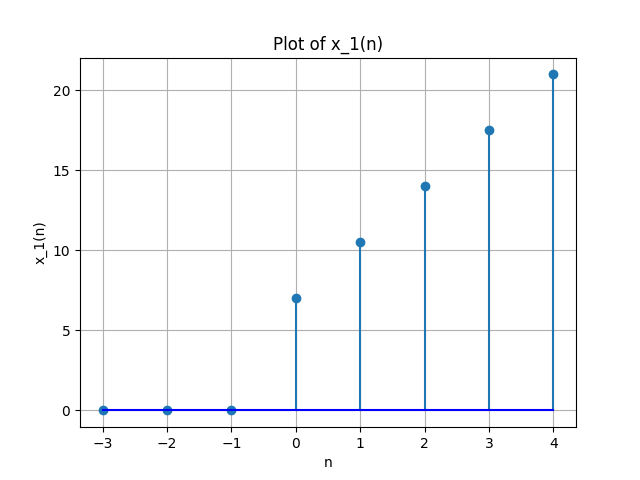
\includegraphics[width=\columnwidth]{graph_1}
\caption{ $y_1\brak{n}$ vs n }
\label{graph:ee25-g2}
\end{figure}
\vspace{0.5cm}


\vspace{0.5cm}
\item
 34 + 32 + 30 ... + 10
\vspace{0.5cm}

\begin{align}
x_2\brak{n} &= \brak{x_2\brak{0} + nd_2}u_{\brak{n}}\\
     10 &= 34 -2n\\
     n &= 12 
     \end{align}

\begin{enumerate}
\item
Z-Transform of $x_2\brak{n}$ :
Using $\eqref{eq:ztrans}$
\begin{align}
X_2(z)&= \frac{34z}{z-1}-
       \frac{2z}{\brak{z-1}^{2}} \label{eq:ee25-6}
,\quad \abs {z}>\abs{1} 
\end{align}


\item
Z-Transform of $y_2\brak{n}$ :
\begin{align}
    y_2\brak{n} &= x_2\brak{n} * h\brak{n} \\
         h\brak{n} &= u\brak{n} \\
         Y_2\brak{z} &= X_2\brak{z} * H\brak{z}\\
        &= \brak{\frac{34z}{\brak{z-1}^{1}}-
       \frac{2z}{\brak{z-1}^2}}\brak{\frac{z}{z-1}}
,\quad \abs {z}>\abs{1} 
    \end{align}

    \item
Inversion of $Y_2\brak{z}$ :
 Using Contour Integration :
\begin{align}
    y_2{(12)}&=\frac{1}{2\pi j}\oint_{C}\brak{\frac{34z^{13}}{\brak{z-1}^2}-
       \frac{2z^{13}}{\brak{z-1}^3}} \;dz 
\end{align}
For $R_1$ , $m=2$ :
\begin{align}
  R_1 &=\frac{1}{\brak {1}!}\lim\limits_{z\to 1}\frac{d}{dz}\brak {{(z-1)}^{2}\frac{34z^{13}}{{(z-1)}^2}}   \\
    &=34\lim\limits_{z\to 1}\frac{d}{dz}(z^{13})   \\
    &= 442
    \end{align}
   For $R_2$ , $m=3$ :
    \begin{align}
    R_2 
&=\frac{1}{\brak {2}!}\lim\limits_{z\to 1}\frac{d^{2}}{dz^{2}}\brak {{(z-1)}^{3}\frac{\brak{-2z^{13}}}{{(z-1)}^3}}   \\
    &=-\lim\limits_{z\to 1}\frac{d^2}{dz^2}(z^{13})   \\
    &= -156\\
    R_1 + R_2 &= 286\\
    \implies  y_2{(12)} &= 286
\end{align}

\end{enumerate}



\begin{figure}[ht!]
\centering
  \graphicspath{ {figs/} }
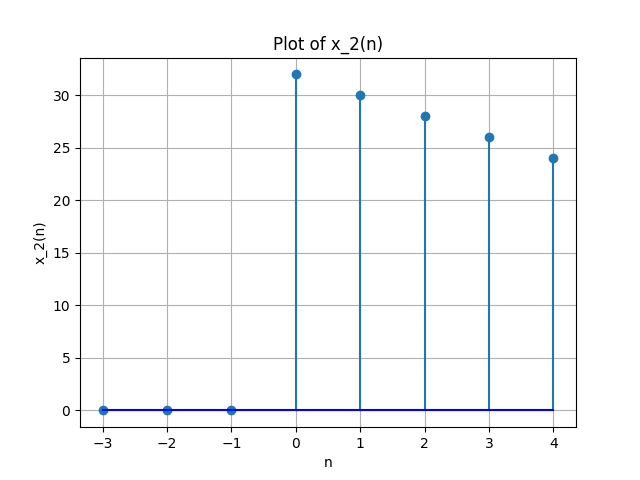
\includegraphics[width=\columnwidth]{graph_2}
\caption{$y_2\brak{n}$ vs n }
\label{graph:ee25-g3}
\end{figure}

\vspace{0.5cm} 
\item
-5 + -8 + -11 ... -230
\vspace{0.5cm}

\begin{align}
x_3\brak{n} &= \brak{x_3\brak{0} -3n}u_{\brak{n}}\\
-230 &= -5 -3n \\
n &= 75
\end{align}
\begin{enumerate}
\item
Z-Transform of $x_3\brak{n}$ :
Using $\eqref{eq:ztrans}$
\begin{align}
X_3\brak{z} &=  \frac{-5z}{\brak{z-1}^{1}} -
       \frac{3z}{\brak{z-1}^{2}} \label{eq:ee25-8}
,\quad \abs {z}>\abs{1} 
\end{align}

    \vspace{0.5cm}
\item
Z-Transform of $y_3\brak{n}$ :
\begin{align}
    y_3\brak{n} &= x_3\brak{n} * h\brak{n} \\
         h\brak{n} &= u\brak{n} \\
    Y_3\brak{z} &= X_3\brak{z} * H\brak{z}\\
             &= \brak{\frac{-5z}{{\brak{z-1}^1}}-
       \frac{3z}{\brak{z-1}^2}}\brak{\frac{z}{z-1}}
,\quad \abs {z}>\abs{1} 
    \end{align}

    \item
Inversion of $Y_3\brak{z}$ :
Using Contour Integration :
\begin{align}
    y_3{(75)}&=\frac{1}{2\pi j}\oint_{C}\brak{\frac{-5z^{76}}{\brak{z-1}^2}-
       \frac{3z^{76}}{\brak{z-1}^3}} \;dz 
\end{align}
For $R_1$ , $m=2$ :
\begin{align}
    R_1 &=\frac{1}{\brak {1}!}\lim\limits_{z\to 1}\frac{d}{dz}\brak {{(z-1)}^{2}\frac{-5z^{76}}{{(z-1)}^2}}   \\
    &=-5\lim\limits_{z\to 1}\frac{d}{dz}(z^{76})   \\
    &= -380
        \end{align}
  For $R_2$ , $m=3$ :
    \begin{align}
    R_2 &=\frac{1}{\brak {2}!}\lim\limits_{z\to 1}\frac{d^{2}}{dz^{2}}\brak {{(z-1)}^{3}\frac{3z^{76}}{{(z-1)}^3}}   \\
    &=1.5\lim\limits_{z\to 1}\frac{d^2}{dz^2}(z^{76})   \\
    &= -8550\\
    R_1 + R_2 &= -8930\\
    \implies  y_3{(75)} &= -8930
\end{align}
    \end{enumerate}



\begin{figure}[ht!]   
\centering
    \graphicspath{ {figs/} }
    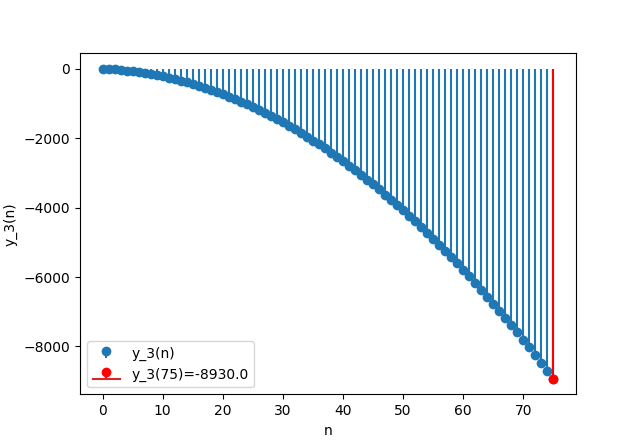
\includegraphics[width=\columnwidth]{graph_3}
    \caption{$y_3\brak{n}$ vs n }
    \label{graph:ee25-g4}
\end{figure}
 \end{enumerate}
\end{document}
